\documentclass[a4paper]{article}
\usepackage[warn]{mathtext}
\usepackage[utf8]{inputenc}
\usepackage[T2A]{fontenc}

\usepackage[english,russian]{babel}
\usepackage{multicol}
\usepackage{fancyhdr}
\usepackage{graphicx}
\usepackage{microtype}
\usepackage{wrapfig}
\usepackage{amsmath}
\usepackage{floatflt}
\usepackage{geometry} \geometry{verbose,a4paper,tmargin=2cm,bmargin=2cm,lmargin=1.5cm,rmargin=1.5cm}
\usepackage{float}
\usepackage{amssymb}
\usepackage{caption}
\usepackage{epsfig}
\usepackage{newunicodechar}

\begin{document}

\graphicspath{ {pictures/} }

\begin{titlepage}
	\centering
	\vspace{5cm}
    {\scshape\LARGE Московский физико-технический институт\par}
	\vspace{5cm}
	{\scshape\Large Лабораторная работа по общей физике \par}
	\vspace{1cm}
    {\huge\bfseries  10.1 Электронный парамагнитный резонанс \par}
	\vspace{1cm}
	\vfill
    \begin{flushright}
        {\large выполнил студент Б04-852 группы ФЭФМ}\par
        \vspace{0.3cm}
        {\LARGE Яромир Водзяновский}
    \end{flushright}
	\vfill
Долгопрудный, 2020
% Bottom of the page
\end{titlepage}

\pagestyle{fancy} 
\fancyhead[L]{Электронный парамагнитный резонанс    $\sim  \hat(\, ^{\circ}  \omega  ^{\circ} \, \hat) \sim$}
\fancyhead[R]{Квантовая физика}
\fancyhead[C]{}
\fancyfoot[C]{ \noindent\rule{\textwidth}{0.4pt} \thepage }

\tableofcontents

\newpage



\section{Цель работы}

\begin{itemize}
    \item Исследовать электронный парамагнитный резонанс в молекуле ДФПГ
    \item Определить $g$-фактор электрона
    \item Измерить ширину линии ЭПР
\end{itemize}



\section{Теория}

Энергетический уровень электрона в присутствии магнитного поля с индукцией $\vec{B}$ расщепляется на два подурвня, расстояние между которыми равно:

\begin{equation}
    \Delta E = E_2 - E_1 = 2 \mu B
\end{equation}

$\mu$- абсолютная величина проекции магнитного момента на направление поля.\par 

Между двумя уровнями возможны переходы. Эти переходы возбуждаются внешним высокочастотным электромагнитным полем, 
если оно имеет нужную частоты (энергия квантов равна расстоянию между уровнями) и нужное направление (магнитный вектор 
перпендикулярен вектору магнитной индукции основного поля $\vec{B}$ или имеет достаточно большую составляющую в указанном 
направлении). \par 

Резонансное значение чатоты определяется из очевидной формулы 

\begin{equation}
    \hbar \omega_0 = \Delta E = 2 \mu B
\end{equation}

При переходе с нижнего уровня на вернхний электрон поглощает квант электромагнитной энергии, 
а при оьратном переходе такой же квант излучается. Возбуждение электронных резонансных переходов электромагнитным путем, 
имеющим частоту, определяемую формулой (2)6 носит название электронного парамагнитног резонанса. \par 

ЭПР возникает из-за поворота спина электронров под действием высокочастотного электромагнитного поля. Не все 
вещества могут совершать такие перевороты. Электроны заполненных оболочек вообще не могут менять своего движения - ни пространственног , ни спинового. 
Сигнал электронного парамагнитного рещонанса наблюждается только на неспаренных электронах, наличие таких электронов приводит 
к парамагнетизму. Так можно исследовать парамагнетики. \par 

Спин-орбитальное взаимодействие. В свободных атомах электрические поля, действующие на атомные электроны, являются центральными, и момент 
количества движения электрона созраняется. В этих условиях орбитальное квантовое число $L$ является 
квантовым числом, сохранение которого обеспечивакется с заметной точностью, а $J$, характеризующее полный момент количества движения, оказывается проктически точным 
квантовым числом. В кристаллах и радикалах дело не так. Поле, дейсвующее на электроны теряет центральный характер и квантовое число, характериующее момент 
количеаства движения отдельного жлектрона, перестает быть точным квантовым числом. Связанные с пространственным движением электронов магнитные поля продолжают 
продолжают вносить вклад в полное поле, действующее на магнитный момент электрона, и влияют на число, положение и форму линий электронного парамагнитного резонанса. 
Возникающая благодаря спин-орбитального взаимодействия тонкая структура линий ползволяет исследовать внутримолекулярные и внутрикристаллические поля. \par 

Рассмотрим структурную формулу ЭПР свободного радикала фенилпикрилгидразила ДФПГ (рис.\ref{matter})

\begin{wrapfigure}[13]{l}{180pt}
    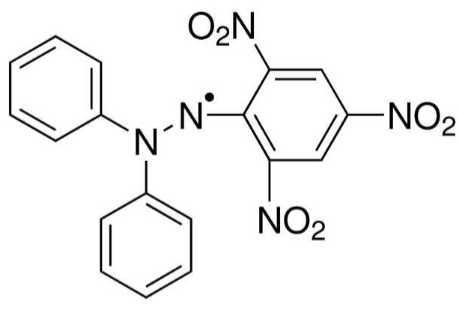
\includegraphics[scale = 0.6]{matter.png}
    \caption{{Химическая структура молекулы ДФПГ}}
    \label{matter}
\end{wrapfigure}

Химичесаая формула $C_{18}H_{12}N_5O_6$, молярная масса 394 г/моль.
Структура на рис. \ref{matter}. В твердом состоянии ДФПГ формуриует твердый кристалл. Исследуемый образец состоит из некоторого 
количества порошка твердого ДФПГ, помещенного в стеклянную ампулу. \par 

Один из электронов центрального атома азота остается неспаренным, резонансное поглощение наблюдается именно на этом электроне. 
Неспаренные электроны радикалов приводят к их повышенной активности.
ДФПГ используется в физике магнитного резонанса как стандартный маркер, позволяющий контролировать точность работы спектрометра. Величина $g$-фактора в ДФПГ 
сотсавляет 2.0036 и с высокой точностью является изотропной. \par 

В молекуле ДФПГ один спин $S = 1/2$ приходится на 41 атом (что делает спины почти свободными), между молекулами в кристалле твердого ДФПГ существует взаимодействие. 
Эксперименты при очень низких температурах показали, что при  температуре 0.3-0.7 К происходит антиферромагнитное упорядочение: направления спинов на соседних молекулах чередуются.\par 

Рассмотрим основыне процессы влиящюие на ширину линии ЭПР. В отсутсвие высокочастотного поля заселенность верхнего и нижнего уровней $N_в$ и $N_н$ 
определяется температурой и описывается обысной формулой Больцмана: 

\begin{equation}
    \frac{N_b}{N_н} = \exp{ \left( -\frac{\Delta E}{k_Б} \right ) }
\end{equation}

В присутсвие резонансного поля между уровнями возникают индуцированные переходы, ведущие к тому, что заселенность верхнего уровня растет, а нижнего падает. 
Этот процесс ведет к нарушению соотношения (3). Востановление теплового равновесия в заселенностях уровней осуществляется благодаря передаче энергии 
возбуждения другим степеням свободы тела. \par 

Эти степени свободы разделяются на две группы: степени свободы, связанные с ориентацией спинов неспаренных электронов, и степени свободы, связанные с 
движением атомов и молекул вещества. Передача энергии в эти степени свободы осуществляется, во-первых, благодаря взаимодействию между магнитным моментом 
рассматриваемого электрона и магнитными моментами других электронов - так называемое спин-спиновое взаимодействие - и, во-вторых, благодаря 
взаимодействию электрона с атомами и молекулами вещества, носящему название спин-решеточного взаимодействия. Эти два взаимодействия легко отличиммы 
экспериментально - различие в температурных зависимостях. В то время как спин-решеточное взаимодействие быстро возрастает с температурой (число фононов), спин-спиновое 
взаимодействие от температуры практически не зависит. \par 

Оба типа взаимодействия способствуют релаксации - переходу из возбужденного состояния в основное - и, следовательно, укорачивают время, которое проводит электрон на верхнем уровне. 
Ширина уровня связана со временем релаксации соотношением неопределенностей:

\begin{equation}
    \Delta E \approx \frac{\hbar}{\tau}, \;\;\;\;\;\;\;\;\; \Delta \omega \frac{1}{\tau}
\end{equation}

Ширина линии поглощения $\Delta \omega$ тем больше, чем меньше время релаксации. \par 

В работе нужно получить сигнал ЭПР на кристаллическом ДФПГ и определить значение $g$-фактора для электрона. 
Как известно, связь между маогнитным моментом $\mu$ электрона и его механическим моментом $M$ выраэается через 
гиромагнитное отношение $\gamma$:

\begin{equation}
    \mu = \gamma M
\end{equation}
 
Если магнитный момент измерять в магнетронах Бора, а механический в единицах $\hbar$, то связь выразится через $g$-фактор:

\begin{equation}
    \frac{\mu}{\mu_Б} = \frac{g M}{\hbar}
\end{equation}

Эта формула справедлива и для соответствующих проекций $\mu$ и $M$ на любое выбранное направление:

\begin{equation}
    \frac{\mu}{\mu_Б} = \frac{g s \hbar}{\hbar}
\end{equation}

$s = 1/2$ - спин электрона. Используя соотношение (2) можно вырахить $g$-фактор через определяемые экспериментальыне величины:

\begin{equation}
    g = \frac{\hbar \omega_0}{\mu_Б B}
\end{equation}

Чисто спиновый характер магнетизма в ДФПГ (практически отсутсвует орбитальный магнетизм) приводит к тому, что парамагнинтый резонанс на неспаренных 
электронах происходит почти как на свободных частицах. ПОэтому $g$-фактор, полученный из электронного 
парамагнитного резонанса в дифенилпикригидразиле, всего на десятые доли процента отличается от $g$-фактора свободного электрона. \par

В методе ЭПР изучается резонансное поглощение переменного электромагнитного поля в образце в зависимости от контролируемых 
экспериментатором внешних условий: постоянного магнитного поля, частоты колебаний переменного поля, температуры... 

\begin{figure}[H]
    \begin{center}
    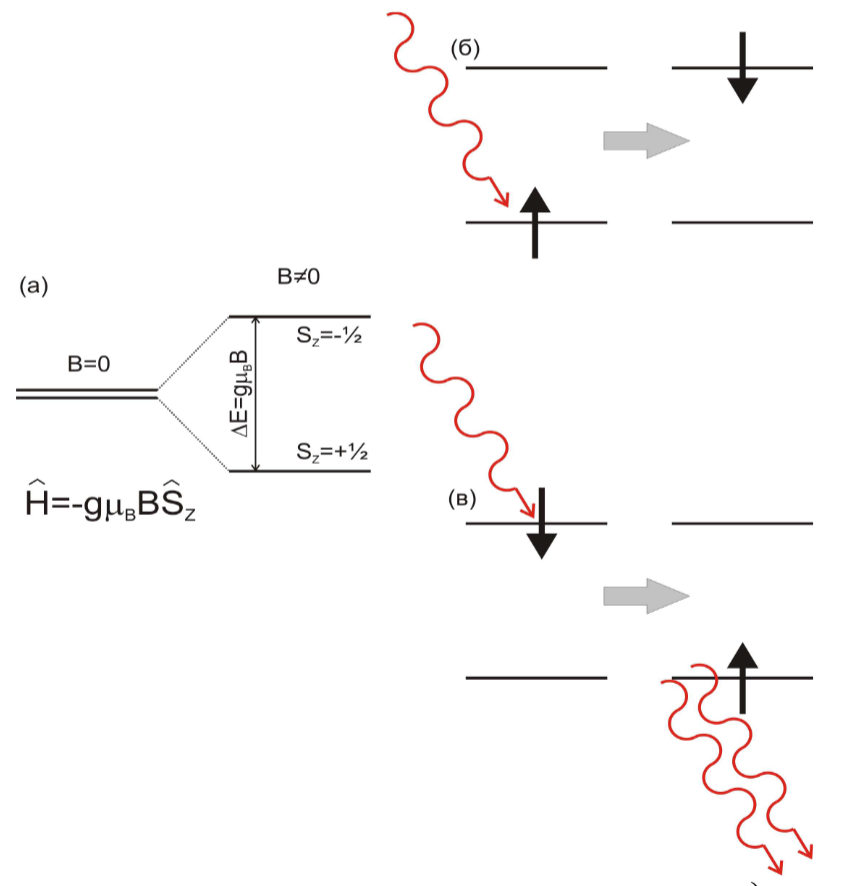
\includegraphics[scale = 0.8]{respogl.png}
    \caption{Схема резонансного поглощения электромагнитного излучения для изолированного спина $S = 1/2$. (a) Зеемановское расщепление спинового уровня в магнитном поле. (б) Переход между подуровнями <<снизу-вверх>> с поглощением фотона резонансной частоты $h \nu = g \mu_B B$. (в) Переход между подуровнями <<сверху-вниз>> с излуением дополнительного фотона резонансной частоты}
    \label{respogl}
    \end{center}
\end{figure}

Простейщей моделью ЭПР есть система невзаимодействующих частиц со спином 1/2, помещенная во внешнее магнитное поле. 
В отсутствие магнитного поля энергии состояний с проекцией спина $S_z = \pm 1/2$ совпадают. Из-за эффекта Зеемана энергии 
состояний с различными проекциями спина начинают различаться (рис. 1а).
Если направить на нашу систему поток излучения (фотонов) с энергией, равной разнице энергий этих состояний $h \nu = g \mu_B B$, то 
станут возможны индуцированные переходы между состояниями. Эти переходы происходят с поглощением (рис. 1б) или 
испусканием (рис. 1в) фотона в зависимости от того, в каком из состояний была система до взаимодействия с излучением.
В отличие от оптических переходов между электронными уровнями энергии в атоме, типичная чатота переменного поля в ЭПР эксперименте 
составляет порядка 10 ГГц (в лабораторном эксперименте 100 МГц)б что соответствует энергии фотона менее 1К. Поэтому, 
за исключением очень низких температур, заселенность обоих спиновых подуровней с $S_z = \pm 1/2$ близка. 
В состоянии теплового равновесия нижний жнергетический уровень более заселен, поэтому наблюдается поглащение  Э-М излучения.



\section{Установка}

Схема представлена на рис. \ref{setup}. Переменное электромагнитное поле на частоте 100 МГц создается 
высокочастотным генератором, постоянное магнитное поле создается электромаогнитом. \par 

Поглощаемая мощность $P_{погл} = \frac{1}{2} \omega b^2 \chi''(\omega, B)$ пропорциональна квадрату амплитуды 
переменного поля $b$. Для увеличения чувствительности эксперимента образец помещают в катушку индуктивности колебательного контура.
Колебательный контур состоит из индуктивности и конденсатора. Еммкость конденсатора изменяется штоком. Генератор 
высокой частоты не соединен с контуром непосредственно: для вощбуждения колебаний в контуре служит электродинамическая связь 
в виде антенны, соединенной с вызодом генератора. Излученное антенной электромагнитное поле возбуждает колебания в контуре. Для 
определения амплитуды этих вынужденных колебаний ряжом с катушкой индуктивности контура расположен виотк с премной катушки детектора. Колебания 
магнитного поля в катушке индуктиыности наводят ЭДС индукции в этом витке. Частота колебаний этов ЭДС индукции соответсвует 100 МГц, для 
измерения этого сигнала он подается на детектор. Детектор - высокочастотгный диод, при малых амплитудах напряжение детектирования происходит за счет нелинейности его ВАХа и 
среднее напряжение на диоде оказывается пропорционально квадрату амплитуды переменного напряжения, то есть квадрату амплитуды переменного свгнитного 
поля в катушке индуктивности, в цепь детектора подключен осциллограф.

\begin{figure}[H]
    \begin{center}
    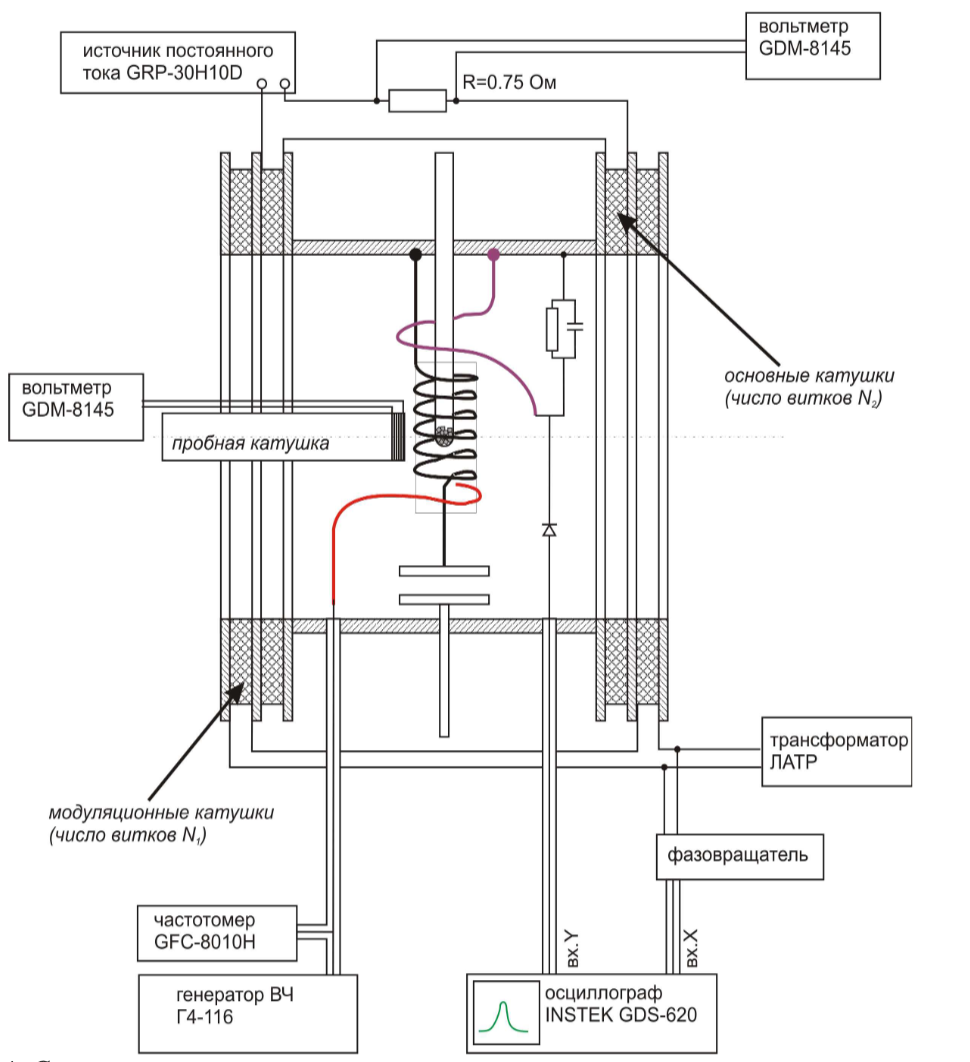
\includegraphics[scale = 0.8]{setup.png}
    \caption{Схема установки}
    \label{setup}
    \end{center}
\end{figure}

Для создания магнитного поля используется электромагнит, состоящий из пары разнесенных катушек. Ток через 
электрормагнит контролируется по падению напряжения на резисторе,включенным в цепь питания катушек. Также имеется 
пара модуляционных катушек, которые могут создавать переменное поле малой апмлитуды. Для создания переменного 
поля к катушкам прикладывается напряжение с трансформатора ЛАТР, частота колебаний переменного поля соответствует частоте колебаний 
напряжения в сети переменного тока. Калибровка электромагнита осуществляется по измерению наводимой ЭДС индукции в пробной 
катушке ищвестной геометрии при подаче переменного тока в соответсвующие катушки электромагнита.  \par 

Для измерений генератор высокой частоты настраивается на резонансную частоту колебаний контура. Амплитуда колебаний 
поля в катушке контура определяется добротностью контура и уменьшится при возникновении поглощения в образце. 
Поэтому необходимо подстроить ток через катушки электромагнита до возникновения этого поглощения. Дополнительная модуляция этого 
поля используется для облегчения настройки.  \par 

Настройка спектрометра на условия резонансного поглощения пощволяет определить эффективный $g$-фактор образца и, 
измерив ширину линии резонансного поглощения, получить информацию о процессах релаксации. \par 

Параметры установки $N_1 = 5850,\; d_1 = 0.23mm \;\;\;\; N_2 = 1260,\; d_2 = 0.3mm \;\;\; N_{проб} = 46, \; d_{проб} = 14.6 \pm 0.1 mm$

\section{Ход работы}

\begin{enumerate}
    \item
    Настроим ВЧ генератор на частоту колебательного контура. \par 
    В режиме непрерывной генерации ВЧ генератор 
    выдает переменный 100 МГц чигнал постоянной амплитуды, который после детектирования превращается в постоянное напряжение. 
    Для удобства настройки сигнал дополнительно модулируется 400 Гц частоте. Детектирование усредняет 
    высокочастотный сигнал, а его огибающая превращается в низкочастотный переменный сигнал, легко визуализируемый на 
    осциллограф. Для наблюдения сигнала переведем осциллограф в режим развертки по времени. По изображению на осциллографе можно определить 
    резонансное значение частоты и значение частот, когда амплитуда уменьшится вдвое. Добротность контура можно 
    определить по формуле:

    \begin{equation}
        Q = \frac{f_0}{f_{+1/2} - f_{-1/2}}
    \end{equation}

    $f_0$ - резонанс, а $f_{-1/2}$ - значение частоты, когда амлитуда упала в два раза.\par 


    \item
    Настроим резонансное поле и определим толщину резонансной кривой.\par 

    Подключим основные катушки к источнику постоянного тока, а модуляционный катушки к трансформатору ЛАТР.
    Осциллограф оставим в режиме развертки по времени, постоянную времени установим так, чтобы на экране было удобно 
    наблюдать сигнал с частотой 50 Гц (трансформатор подключен к розетке). ВЧ-генератор переведем в режим
    непрерывной генерации, на канале осциллографа, подключенном к детектору, устанвоим максималную чувствительтность. \par 

    Подадим на модуляционный катушки напряжение 50 В (по вольтметру на ЛАТР).  Плавно увеличивая постоянное напяржение, подаваемое на основные катушки
    добьемся возникновения на экране осциллографа картины резонансного поглощения. \par 

    Для боле точной настройки и определения ширины линии резонансного поглощения подадим на Х-канал осциллографа  напряжение 
    прикладываемое к модуляционным катушкам и будем наблюдать сигнал в XY-режиме. На экране будет наблюдаться зависимость поглощения 
    в образце от приложенного переменного поля. При точной настройке постоянного поля наблюдаемая картина должна быть симметрична относительно 
    средней вертикальной оси. Из-за набегающей в электрической схеме расфазировки напряжений на экране наблюдается два пика, соответствующие прохождению 
    резонансного поглощения на растущем и падающем полупериодах модулирующего напряжения, подаваемого на канал X относительно фазы модулирующего напряжения, и 
    позволяет совместить пики.

    \begin{figure}[H]
        \begin{center}
        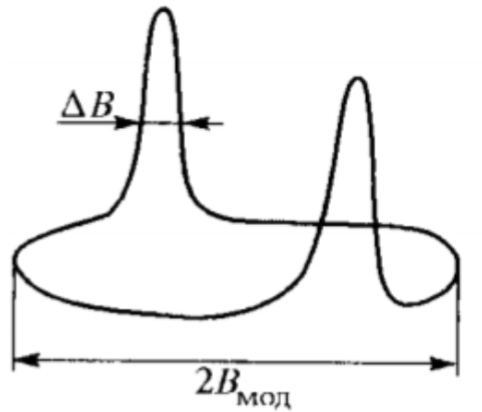
\includegraphics[scale = 0.8]{signal.png}
        \caption{Вид сигнала при расфазировке}
        \label{signal}
        \end{center}
    \end{figure}

    Для определения ширины линии ЭПР определим по экрану осциллографа полный размах модулирующего поля 
    (в делениях шкалы) и полную ширину кривой резонансного поглощения на полувысоте $A_{1/2}$. Не изменяя настроек возьмем
    пробную катушку и внесем её внутрь соленоида максимально близко к образцу. Переменное поле модуляционных катушек 
    наводит в пробной катушке ЭДС индукции, по которой можно определить величину поля. По измеренной ЭДС индукции $\varepsilon_i$ 
    определим амплитуду модулиющего поля:
    
    \begin{equation}
        B_{мод} = \sqrt{2} \frac{2 \varepsilon_i}{\pi^2 d_{проб}^2 N_{проб} \nu}
    \end{equation}

    где $\nu = 400 Гц$ - частота модулиующего напряжения.
    Тогда:
    $$B_{мод} \approx 0.74 мТл$$ 
    Полуширина на полувысоте линии резонанснрго поглощения 
    (в единицах поля) может быть получена как:

    \begin{equation}
        \Delta B = \frac{A_{1/2}}{A_{полн}} B_{мод} \approx 0.064\;мТл
    \end{equation}


    \item Откалибруем электромагнит, определим $g$-фактор. \par 
    Для проведения калибровочных измерений подключим основные катушки на ЛАТР. Это делается коммутацией переключателя.
    Переведем вольтметр, измеряющий напряжение на резисторе в цепи основных катушек в режим измерений на переменном токе.
    Установим ток через катушки, близкий к значению тока при наблюдении резонансного поглощения, и измерим в этих условиях ЭДС 
    индукции в пробной катушке. Для контроля однородности поля внесем катушку в центр магнита с передней и задней стороны установки. 
    Проведем калибровочные измерения $\approx 20 $ значений напряжения в интервале $\pm 15$ мВ от значения напряжения, зафиксированного 
    в условиях резонансного поглощения. \par 

    С помощью пробной катушки определим индукцию магнитного поля из:

    \begin{equation}
        V = nB_0S\omega = \frac{\pi}{4} n B_0 d^2\omega \rightrightarrows B_0 = \frac{4V}{\pi n d^2 \omega}
    \end{equation}

    Получим остюда:

    $$B_0 \approx 1.05 \; мТл$$

    $g$-фактор поределим по формуле:

    \begin{equation}
        g = \frac{\hbar \omega_0}{\mu_Б} \approx 1.9
    \end{equation}
\end{enumerate}



\section{Вывод}
В ходе эксперимента было исследовано явление ЭПР на молекуле ДФПГ и получены значения полуширины линии ЭПР и значение $g$-фактора.
В целом значения в каком-то приближении близки к табличным: 
$$\Delta B \approx 0.064\;[мТл],\;\;\;\; g \approx 1.9 $$
Табличные значения: 
$$\Delta B = 0.010-0.015\; [мТл],\;\;\;\;\; g = 2.0036$$
\end{document}